\documentclass{article}


\usepackage[T1]{fontenc}
\usepackage{graphicx}
\usepackage[bookmarks,unicode,colorlinks=true,breaklinks=true]{hyperref}
\usepackage{color}
\usepackage[a4paper,margin=1cm,footskip=0.25in]{geometry}

\usepackage{xspace}
\usepackage[tableposition=top]{caption}
\usepackage{wrapfig}

\usepackage{amssymb}
\usepackage{mathtools}
\usepackage{microtype}

\usepackage{booktabs}
\usepackage{caption}
\usepackage{subfigure}
\usepackage{multicol}
\usepackage{xifthen}
\usepackage{etoolbox}
\usepackage{tikz}
\usetikzlibrary{arrows,shapes,calc,automata,positioning}
%\tikzset{align at top/.style={baseline=(current bounding box.north)}}
%\tikzstyle{every node}=[font=\scriptsize]
\tikzstyle{state} = [draw,fill=white,circle,thick,align=center,inner sep=0pt,minimum size=4.5mm]
\tikzstyle{lstate} = [draw,fill=white,rectangle,rounded corners,thick,align=center,inner sep=2pt]
\tikzstyle{dot} = [fill,circle,inner sep=0mm,minimum size=1.25mm,line width=0mm]

\usepackage{pgfplots}
\pgfplotsset{compat=newest}

%\usepackage{todonotes}

\usetikzlibrary{shapes,positioning,arrows,calc,automata,matrix,fit}
\newcommand{\drawcirc}{\node[draw,circle,minimum size=.7cm, outer sep=1pt]}
\newcommand{\drawbox}{\node[draw,rectangle,minimum size=.7cm, outer sep=1pt]}
\newcommand{\drawdummy}{\node[minimum size=0,inner sep=0]}
\usepackage{xfrac}

\usepackage[capitalise]{cleveref}
\Crefname{equation}{Eq.}{Eqs.}
\Crefname{figure}{Fig.}{Figs.}
\Crefname{tabular}{Tab.}{Tabs.}
\Crefname{remark}{Rem.}{Rems.}
\Crefname{section}{Sec.}{Secs.}
\Crefname{subsection}{Sec.}{Secs.}
\Crefname{proposition}{Prop.}{Props.}
\usepackage{csquotes} % for enquote

% Spacing between text and display math
\makeatletter%
\g@addto@macro\normalsize{%
  \setlength\abovedisplayskip{3pt}%
  \setlength\belowdisplayskip{3pt}%
  \setlength\abovedisplayshortskip{-3pt}%
  \setlength\belowdisplayshortskip{3pt}%
}%
\makeatother
%\renewcommand{\baselinestretch}{0.974} % >=0.97
%
\renewcommand{\paragraph}[1]{\smallskip\noindent\emph{#1}}

% MDP definition
\newcommand{\mdp}{\mathcal{M}}
\newcommand{\states}{\mathsf{S}}
\newcommand{\actions}{\mathsf{A}}
\newcommand{\trans}{\delta}

% General math
\newcommand{\dist}{\mathsf{d}}
\newcommand{\dists}{\mathsf{D}}
\newcommand{\eqdef}{\vcentcolon=}
\newcommand{\Rationals}{\mathbb{Q}}
\DeclareMathSymbol{\sm}{\mathbin}{AMSa}{"39} % short minus
\newcommand{\set}[1]{\ensuremath{\{\,#1\,\}}}
\newcommand{\tuple}[1]{\ensuremath{( #1 )}}

% Semantics
\newcommand{\apath}{\rho}
\newcommand{\policy}{\pi}
\newcommand{\policies}{\Pi}
\newcommand{\paths}{\mathsf{Paths}}
\newcommand{\prob}{\mathbb{P}}

% Objectives
\newcommand{\reachObj}{\mathsf{R}}
\newcommand{\ERObj}{\mathsf{E}}
\newcommand{\initstate}{s_i}
\newcommand{\targets}{\mathsf{T}}
\newcommand{\opt}{\mathsf{opt}}
\renewcommand{\min}{\ensuremath{\mathrm{min}}}
\renewcommand{\max}{\ensuremath{\mathrm{max}}}
\newcommand{\val}{\mathsf{V}}
\newcommand{\rew}{\mathsf{rew}}
\newcommand{\Pobj}[2]{\ensuremath{\mathrm{P}_{{\!}#1}(#2)}}
\newcommand{\Eobj}[2]{\ensuremath{\mathrm{E}_{#1}(#2)}}
\newcommand{\Pmin}{\ensuremath{\mathrm{P}_{\min}}\xspace}
\newcommand{\Pmax}{\ensuremath{\mathrm{P}_{\max}}\xspace}

% For LP
\newcommand{\lowerbound}{lb}
\newcommand{\upperbound}{ub}

% Abbreviations
\newcommand{\ie}{i.e.\xspace}
\newcommand{\eg}{e.g.\xspace}
\newcommand{\wrt}{w.r.t.\xspace}
\newcommand{\cf}{cf.\xspace}
\newcommand{\etal}{et al.\xspace}
\newcommand{\qee}{\hfill $\vartriangle$}

% Tools etc.
\newcommand{\tool}[1]{\textsf{#1}\xspace}
\newcommand{\storm}{\tool{Storm}}
\newcommand{\mcsta}{\tool{mcsta}}
\newcommand{\solver}[1]{\textsf{#1}\xspace}

% Better checkmark and x-mark
\usepackage{pifont}% http://ctan.org/pkg/pifont
\newcommand{\cmark}{\text{\ding{51}}}%
\newcommand{\xmark}{\text{\ding{55}}}%


\newcommand{\comset}{\textit{practitioner-set-2024}\xspace}
\newcommand{\Direct}{Common\xspace}
\newcommand{\direct}{common\xspace}
\newcommand{\Modifying}{WORD2\xspace}
\newcommand{\modifying}{wORD2\xspace}

\newcommand{\changed}[1]{#1}

% Commands for Plots
% outdated (from TACAS)
\newcommand{\numqvbsfull}{366}
\newcommand{\numqvbshard}{18}


\newcommand{\numcommunity}{80}
\newcommand{\numpremise}{200}
\newcommand{\numalljani}{449}
\newcommand{\numhard}{117}
\newtoggle{showplots}
 \toggletrue{showplots}
% \togglefalse{showplots}
 % \usepackage{showframe}

%% Colours
\definecolor{plotred}{RGB}{255,0,0}
\definecolor{plotgreen}{RGB}{0,255,0}
\definecolor{plotblue}{RGB}{0,0,255}
\definecolor{plotyellow}{RGB}{230,230,0}
\definecolor{plotcyan}{RGB}{0,255,255}
\definecolor{plotorange}{RGB}{255,127,0}
\definecolor{plotpink}{RGB}{255,0,255}
\definecolor{plotlightgray}{RGB}{192,192,192}
\definecolor{plotdarkgray}{RGB}{128,128,128}
\definecolor{plotdarkred}{RGB}{128,0,0}
\definecolor{plotgreenyellow}{RGB}{128,128,0}
\definecolor{plotdarkgreen}{RGB}{0,128,0}
\definecolor{plotpurple}{RGB}{128,0,128}
\definecolor{plotteal}{RGB}{0,128,128}
\definecolor{plotdarkblue}{RGB}{0,0,128}
\definecolor{plotlightred}{RGB}{205,92,92}
\definecolor{plotlightblue}{RGB}{176,196,222}
\colorlet{color1}{plotred}
\colorlet{color2}{plotgreen}
\colorlet{color3}{plotblue}
\colorlet{color4}{plotyellow}
\colorlet{color5}{plotcyan}
\colorlet{color6}{plotorange}
\colorlet{color7}{plotpink}
\colorlet{color8}{plotlightgray}
\colorlet{color9}{plotdarkgray}
\colorlet{color10}{plotdarkred}
\colorlet{color11}{plotgreenyellow}
\colorlet{color12}{plotdarkgreen}
\colorlet{color13}{plotpurple}
\colorlet{color14}{plotteal}
\colorlet{color15}{plotdarkblue}
\colorlet{color16}{plotlightred}
\colorlet{color17}{plotlightblue}

\colorlet{colmcstavi}{color1}
\colorlet{colmcstaovi}{color11}
\colorlet{colstormvi}{color3}
\colorlet{colstormovi}{color7}
\colorlet{colstormpi}{color14}
\colorlet{colstormlp}{color6}



%% Quantileplots
\newcommand{\quantileplotxlabel}{solved benchmarks}
\newcommand{\quantileplotylabel}{runtime}
\newlength{\quantileplotwidth}
\newlength{\quantileplotheight}
\setlength{\quantileplotwidth}{0.5\linewidth}
\setlength{\quantileplotheight}{0.5\linewidth}
\newcommand{\quantileplotlegendcols}{1}

\newcommand{\standardquantileplotlinestyle}{ultra thick}
\newcommand{\quantileplotlinestyle}{\standardquantileplotlinestyle}

\newcommand{\quantileplot}[8]{%
% Arguments:
% #1: csv filename
% #2: comma separated list of tool.config/color items}
% #3: comma separated list of readable config names 
% #4: xmin
% #5: xmax
% #6: ymin
% #7: ymax
% #8: legend pos (e.g. "north west")
	\begin{tikzpicture}
	\begin{axis}[
	width=\quantileplotwidth,
	height=\quantileplotheight,
	xmin=#4,
	xmax=#5,
	ymin=#6,
	ymax=#7,
	ymajorgrids,
	ymode=log,
	axis x line=bottom,
	axis y line=left,
	unbounded coords=discard,filter discard warning=false, % properly deal with missing data points
	% ytick= {1, 6, 60, 600, 1200, 1800 },
	% yticklabels={$\le$1, 6, 60, 600, 1200, 1800},
	xlabel=\quantileplotxlabel,
	xlabel style={font=\scriptsize,yshift=4pt},%{yshift=16pt},
	ylabel=\quantileplotylabel,
	ylabel style={font=\scriptsize,yshift=-7pt},%{yshift=-0.4cm},
	log ticks with fixed point, % enable to avoid 10^-x notation
	yticklabel style={font=\scriptsize},
	scaled y ticks=false,
	xticklabel style={font=\scriptsize},
	legend columns=\quantileplotlegendcols,
	legend pos={#8},
	legend style={nodes={scale=0.75, transform shape},inner sep=1pt},
/pgfplots/legend image code/.code={\draw[mark repeat=2,mark phase=2,##1] plot coordinates {(0cm,0cm) (0.3cm,0cm)};}, % make the legend lines a bit smaller
	every axis plot/.append style={\quantileplotlinestyle},
	legend cell align={left}
	]
	\iftoggle{showplots}{
	\foreach \tool\color in {#2}{%
		\edef\loopbody{
			\noexpand\addplot[\color] table [x=n,y=\tool shifted, col sep=tab] {#1};
		}
		\loopbody
	}
	\legend{#3}}{\node[anchor=south west, align=center, red] {\huge NOT\\ COMPILED};}
	\end{axis}
	\end{tikzpicture}%
}


%% Scatter plots
\newlength\scatterplotsize
\setlength{\scatterplotsize}{0.365\linewidth}
\newcommand{\scatterplot}[6]{%
% Arguments:
% #1: csv filename
% #2: tool.config identifier for x-axis
% #3: label for x-axis
% #4: tool.config identifier for y-axis
% #5: label for y-axis
% #6: trigger showing the legend (true/false)
	\begin{tikzpicture}
	\begin{axis}[
	width=\scatterplotsize,
	height=\scatterplotsize,
	axis equal image,
	xmin=1,
	ymin=1,
	ymax=1280,
	xmax=1280,
	xmode=log,
	ymode=log,
	axis x line=bottom,
	axis y line=left,
	xtick={2,4,8,16,32,64,128,256},
	xticklabels={2,4,8,16,,64,,\!\!256},
	extra x ticks = {1,512,724},
	extra x tick labels = {${\le}1$,,\,\,n/a},
	extra x tick style = {grid = major},
	ytick={2,4,8,16,32,64,128,256},
	yticklabels={2,4,8,16,32,64,,},
	extra y ticks = {1,512,724},
	extra y tick labels = {${\le}1$,$\ge$512},
	extra y tick style = {grid = major},
	xlabel={#3},
	xlabel style={font=\scriptsize,yshift=5pt},%{yshift=16pt},
	ylabel={#5},
	ylabel style={font=\scriptsize,yshift=-9pt},%{yshift=-0.4cm},
	yticklabel style={font=\scriptsize},
	xticklabel style={font=\scriptsize},%rotate=290,anchor=west,
	legend pos=north east,
	legend columns=3,
	legend style={nodes={scale=0.75, transform shape},inner sep=1.5pt, xshift=1mm, yshift=7mm},
	set layers,
	mark layer=axis background
	%legend cell align={left}
	]
	
	\iftoggle{showplots}{\addplot[
	scatter,
	only marks,
	scatter/classes={
		maqvbs={mark=diamond*,color1,mark size=1.75},
		ptaqvbs={mark=pentagon*,color3,mark size=1.75},
		mdpqvbs={mark=triangle*,color2,mark size=1.75},
		mdpmec={mark=asterisk,color7,mark size=1.75},
		mdpgrid={mark=*,color5,mark size=1.75},
		mdpgridmec={mark=otimes,color6,mark size=1.75}
	},
	scatter src=explicit symbolic
	]%
	table [col sep=tab,x=#2,y=#4,meta=Class] {#1};
	}{\node[anchor=south west, align=center, red] {\huge NOT\\ COMPILED};}
	\ifthenelse{\NOT\equal{#6}{false}}{\legend{MA,PTA,MDP$_\mathit{qvbs}$,MDP$^\mathit{mec}$,MDP$_\mathit{grid}$,MDP$_\mathit{grid}^\mathit{mec}$}}{}
	\addplot[no marks] coordinates {(0.01,0.01) (512,512) };
	\addplot[no marks, densely dotted] coordinates {(0.01,0.02) (256,512)};
	\addplot[no marks, densely dotted] coordinates {(0.02,0.01) (512,256)};
	\end{axis}
	\end{tikzpicture}
}


\newcommand{\hardwarquantileplot}[7]{
% Arguments:
% #1: csv filename
% #2: hardware-config-name
% #4: xmin
% #5: xmax
% #6: ymin
% #7: ymax
% #8: legend pos (e.g. "north west")
\renewcommand{\quantileplotlinestyle}{thick}%
\quantileplot{#1}{#2.Storm.ovi-topo/colstormovi,#2.Storm.vi-topo/colstormvi,#2.mcsta.ovi/colmcstaovi,#2.mcsta.vi/colmcstavi,#2.Storm.vi2pi-topo-gmres/colstormpi,#2.Storm.vi2lp-topo-gurobi/colstormlp}{
%$\text{OVI}_\tool{s}$, $\text{VI}_\tool{s}$, $\text{OVI}_\tool{m}$, $\text{VI}_\tool{m}$,$\text{VI2PI}_\tool{s}$,  $\text{VI2LP}_\tool{s}$
}{#3}{#4}{#5}{#6}{#7}
% Arguments:
% #1: csv filename
% #2: comma separated list of tool.config/color items}
% #3: comma separated list of readable config names 
% #4: xmin
% #5: xmax
% #6: ymin
% #7: ymax
% #8: legend pos (e.g. "north west")
\renewcommand{\quantileplotlinestyle}{\standardquantileplotlinestyle} %
}

\colorlet{colclaix23}{red}
\colorlet{cole1620}{blue!50!white}
\colorlet{colR32200}{green!80!white}
\colorlet{colR54650U}{green!60!black}
\colorlet{colR97950}{green!80!black}
\colorlet{colTRP5965}{green!60!yellow!30!black}
\colorlet{coli910980}{blue!80!white}
\colorlet{coli911900}{blue!90!black}

\colorlet{colM2Pro}{brown}

\newcommand{\hardwarmethodsquantileplot}[7]{
% Arguments:
% #1: csv filename
% #2: method-name
% #4: xmin
% #5: xmax
% #6: ymin
% #7: ymax
% #8: legend pos (e.g. "north west")
\renewcommand{\quantileplotlinestyle}{thick}%
\quantileplot{#1}{logs-E1620-dockerized.#2/cole1620,logs-R32200-dockerized.#2/colR32200,logs-R54650U-dockerized.#2/colR54650U,logs-R97950X-dockerized.#2/colR97950,logs-i910980xe-dockerized.#2/coli910980,logs-M2Pro.#2/colM2Pro,logs-TRP5965-dockerized.#2/colTRP5965,logs-i911900K-dockerized.#2/coli911900,logs-claix23.#2/colclaix23
}{%claix23,E1620,R32200,R54650U,R97950X,TRP5965,i910980,i911900
}{#3}{#4}{#5}{#6}{#7}%
% Arguments:
% #1: csv filename
% #2: comma separated list of tool.config/color items}
% #3: comma separated list of readable config names 
% #4: xmin
% #5: xmax
% #6: ymin
% #7: ymax
% #8: legend pos (e.g. "north west")
\renewcommand{\quantileplotlinestyle}{\standardquantileplotlinestyle} %
}
\newcommand{\hardwaremethodslegend}{
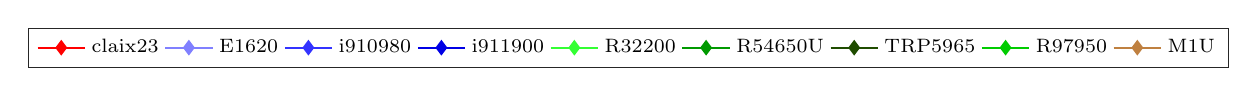
\begin{tikzpicture}
\begin{axis}[width=0.8\textwidth, height=0.2\textwidth, hide axis, xmin=0, xmax=10, ymin=0, ymax=0.2,legend columns=9, 
            legend style={draw=white!15!black,legend cell align=left, at={(0.5,0.5), font=\scriptsize}},]
%    \foreach \toolname/\tcolor in {claix23/colclaix23,E1620/cole1620,i910980xe/coli910980,i911900K/coli911900,R32200/colR32200,R54650U/colR54650U,TRP5965/colTRP5965,R97950X/colR97950}{
%		\edef\loopbody{
%			\noexpand\addlegendimage{\tcolor, mark=diamond*, thick, mark options={solid,scale=1.1}}\noexpand\addlegendentry{\toolname}
%   % what
%		}
%		\show\loopbody
%		\loopbody
%	}
	% claix23/colclaix23,E1620/cole1620,i910980xe/coli910980,i911900K/coli911900,R32200/colR32200,R54650U/colR54650U,TRP5965/colTRP5965,R97950X/colR97950
	\addlegendimage{colclaix23, mark=diamond*, thick, mark options={solid,scale=1.1}}
	\addlegendentry{claix23}
	
	\addlegendimage{cole1620, mark=diamond*, thick, mark options={solid,scale=1.1}}
	\addlegendentry{E1620}
	
	\addlegendimage{coli910980, mark=diamond*, thick, mark options={solid,scale=1.1}}
	\addlegendentry{i910980}
	
	\addlegendimage{coli911900, mark=diamond*, thick, mark options={solid,scale=1.1}}
	\addlegendentry{i911900}
	
	\addlegendimage{colR32200, mark=diamond*, thick, mark options={solid,scale=1.1}}
	\addlegendentry{R32200}
	
	\addlegendimage{colR54650U, mark=diamond*, thick, mark options={solid,scale=1.1}}
	\addlegendentry{R54650U}
	
	\addlegendimage{colTRP5965, mark=diamond*, thick, mark options={solid,scale=1.1}}
	\addlegendentry{TRP5965}
	
	\addlegendimage{colR97950, mark=diamond*, thick, mark options={solid,scale=1.1}}
	\addlegendentry{R97950}
	
	\addlegendimage{colM2Pro, mark=diamond*, thick, mark options={solid,scale=1.1}}
	\addlegendentry{M1U}
	
    \end{axis}
\end{tikzpicture}
}

\newcommand{\hardwarescatterplot}[6]{%
% Arguments:
% #1: csv filename
% #2: tool.config identifier for x-axis
% #3: label for x-axis
% #4: tool.config identifier for y-axis
% #5: label for y-axis
% #6: trigger showing the legend (true/false)
	\begin{tikzpicture}
	\begin{axis}[
	width=\scatterplotsize,
	height=\scatterplotsize,
	axis equal image,
	xmin=1,
	ymin=1,
	ymax=1280,
	xmax=1280,
	xmode=log,
	ymode=log,
	axis x line=bottom,
	axis y line=left,
	xtick={2,4,8,16,32,64,128,256},
	xticklabels={2,4,8,16,,64,,\!\!256},
	extra x ticks = {1,512,724},
	extra x tick labels = {${\le}1$,,\,\,n/a},
	extra x tick style = {grid = major},
	ytick={2,4,8,16,32,64,128,256},
	yticklabels={2,4,8,16,32,64,,},
	extra y ticks = {1,512,724},
	extra y tick labels = {${\le}1$,$\ge$512},
	extra y tick style = {grid = major},
	xlabel={#3},
	xlabel style={font=\scriptsize,yshift=5pt},%{yshift=16pt},
	ylabel={#5},
	ylabel style={font=\scriptsize,yshift=-9pt},%{yshift=-0.4cm},
	yticklabel style={font=\scriptsize},
	xticklabel style={font=\scriptsize},%rotate=290,anchor=west,
	legend pos=north east,
	legend columns=3,
	legend style={nodes={scale=0.75, transform shape},inner sep=1.5pt, xshift=1mm, yshift=7mm},
	set layers,
	mark layer=axis background,
	mark options={scale=0.6}
	%legend cell align={left}
	]
	
	\iftoggle{showplots}{%
	\addplot+[%
	scatter,
	only marks,
		%scatter src=explicit symbolic,
		scatter/use mapped color={draw=colstormovi,fill=colstormovi},mark=diamond*]%
	table [col sep=tab,x=#2.Storm.ovi-topo,y=#4.Storm.ovi-topo] {#1};
	\addplot+[%
	scatter,
	only marks,
		%scatter src=explicit symbolic,
		scatter/use mapped color={draw=colstormvi,fill=colstormvi}, mark=diamond*]%
	table [col sep=tab,x=#2.Storm.vi-topo,y=#4.Storm.vi-topo] {#1};
	\addplot+[%
	scatter,
	only marks,
		%scatter src=explicit symbolic,
		scatter/use mapped color={draw=colmcstaovi,fill=colmcstaovi},mark=*]%
	table [col sep=tab,x=#2.mcsta.ovi,y=#4.mcsta.ovi] {#1};
	\addplot+[%
	scatter,
	only marks,
		%scatter src=explicit symbolic,
		scatter/use mapped color={draw=colmcstavi,fill=colmcstavi}, mark=*]%
	table [col sep=tab,x=#2.mcsta.vi,y=#4.mcsta.vi] {#1};
	\addplot+[%
	scatter,
	only marks,
		%scatter src=explicit symbolic,
		scatter/use mapped color={draw=colstormlp,fill=colstormlp},
		color=blue, mark=pentagon*]%
	table [col sep=tab,x=#2.Storm.vi2lp-topo-gurobi,y=#4.Storm.vi2lp-topo-gurobi] {#1};
	\addplot+[%
	scatter,
	only marks,
		%scatter src=explicit symbolic,
		scatter/use mapped color={draw=colstormpi,fill=colstormpi},
		color=blue, mark=triangle*]%
	table [col sep=tab,x=#2.Storm.vi2pi-topo-gmres,y=#4.Storm.vi2pi-topo-gmres] {#1};
	
%	\addplot+[%
%	scatter,
%	only marks,
%		%scatter src=explicit symbolic,
%		scatter/use mapped color={draw=none,fill=green},
%		color=blue, mark=diamond*]%
%	table [col sep=tab,x=#2.Storm.vi2lp-topo-gurobi,y=#4.Storm.vi2lp-topo-gurobi] {#1};
%	}%
%	\addplot+[%
%	scatter,
%	only marks,
%		%scatter src=explicit symbolic,
%		scatter/use mapped color={draw=none,fill=black},
%		color=blue, mark=diamond*]%
%	table [col sep=tab,x=#2.mcsta.ovi-topo,y=#4.mcsta.ovi-topo] {#1};
	}{\node[anchor=south west, align=center, red] {\huge NOT\\ COMPILED};}
	\ifthenelse{\NOT\equal{#6}{false}}{\legend{$\text{OVI}_\tool{s}$, $\text{VI}_\tool{s}$,  $\text{VI2LP}_\tool{s}$, $\text{VI2PI}_\tool{s}$, $\text{OVI}_\tool{m}$, $\text{VI}_\tool{m}$}}{}
	\addplot[no marks] coordinates {(0.01,0.01) (512,512) };
	\addplot[no marks, densely dotted] coordinates {(0.01,0.02) (256,512)};
	\addplot[no marks, densely dotted] coordinates {(0.02,0.01) (512,256)};
	\end{axis}
	\end{tikzpicture}
}



\newcommand{\scatterplotseb}[6]{%
% Arguments:
% #1: csv filename
% #2: tool.config identifier for x-axis
% #3: label for x-axis
% #4: tool.config identifier for y-axis
% #5: label for y-axis
% #6: trigger showing the legend (true/false)
	\begin{tikzpicture}
	\begin{axis}[
	width=\scatterplotsize,
	height=\scatterplotsize,
	axis equal image,
	xmin=1,
	ymin=1,
	ymax=1280,
	xmax=1280,
	xmode=log,
	ymode=log,
	axis x line=bottom,
	axis y line=left,
	xtick={2,4,8,16,32,64,128,256},
	xticklabels={2,4,8,16,,64,,\!\!256},
	extra x ticks = {1,512,724},
	extra x tick labels = {${\le}1$,,\,\,n/a},
	extra x tick style = {grid = major},
	ytick={2,4,8,16,32,64,128,256},
	yticklabels={2,4,8,16,32,64,,},
	extra y ticks = {1,512,724},
	extra y tick labels = {${\le}1$,$\ge$512},
	extra y tick style = {grid = major},
	xlabel={#3},
	xlabel style={font=\scriptsize,yshift=5pt},%{yshift=16pt},
	ylabel={#5},
	ylabel style={font=\scriptsize,yshift=-9pt},%{yshift=-0.4cm},
	yticklabel style={font=\scriptsize},
	xticklabel style={font=\scriptsize},%rotate=290,anchor=west,
	legend pos=north east,
	legend columns=3,
	legend style={nodes={scale=0.75, transform shape},inner sep=1.5pt, xshift=1mm, yshift=7mm},
	set layers,
	mark layer=axis background
	%legend cell align={left}
	]
	
	\iftoggle{showplots}{
	\addplot+[%
	scatter,
	only marks,
		%scatter src=explicit symbolic,
		scatter/use mapped color={draw=red,fill=red},
		color=red, mark=diamond*]%
	table [col sep=tab,x=#2.Storm.vi2lp-topo-gurobi,y=#2.Storm.vi2pi-topo-gmres] {#1};
	\addplot+[%
	scatter,
	only marks,
		%scatter src=explicit symbolic,
		scatter/use mapped color={draw=blue,fill=blue},
		color=blue, mark=diamond*]%
	table [col sep=tab,x=#4.Storm.vi2lp-topo-gurobi,y=#4.Storm.vi2pi-topo-gmres] {#1};
	}{\node[anchor=south west, align=center, red] {\huge NOT\\ COMPILED};}
	\ifthenelse{\NOT\equal{#6}{false}}{\legend{#2,#4}}{}
	\addplot[no marks] coordinates {(0.01,0.01) (512,512) };
	\addplot[no marks, densely dotted] coordinates {(0.01,0.02) (256,512)};
	\addplot[no marks, densely dotted] coordinates {(0.02,0.01) (512,256)};
	\end{axis}
	\end{tikzpicture}
}



\newcommand{\simplehardwarquantileplot}[1]{%
\hardwarquantileplot{plotdata/quantile-hardware.csv}{logs-#1}%
		{0}{\numcommunity}{0.1}{800}{north west}
	}
	
	\newcommand{\simplehardwaremethodsquantileplot}[1]{
	\hardwarmethodsquantileplot{plotdata/quantile-hardware.csv}{#1}%
		{0}{\numcommunity}{1}{800}{north west}
	}
	
	\newcommand{\hardwareexperimentlegend}{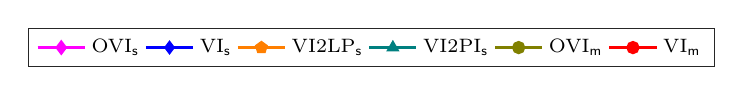
\begin{tikzpicture}
\begin{axis}[width=0.8\textwidth, height=0.2\textwidth, hide axis, xmin=0, xmax=10, ymin=0, ymax=0.2,legend columns=6, 
            legend style={draw=white!15!black,legend cell align=left, at={(0.5,0.5), font=\scriptsize}},]
    \addlegendimage{colstormovi, mark=diamond*, thick, mark options={solid,scale=1.1}}
    \addlegendentry{$\text{OVI}_\tool{s}$}
    \addlegendimage{colstormvi, mark=diamond*, thick}
    \addlegendentry{$\text{VI}_\tool{s}$}
    \addlegendimage{colstormlp, mark=pentagon*, thick}
    \addlegendentry{$\text{VI2LP}_\tool{s}$}
    \addlegendimage{colstormpi, mark=triangle*, thick}
    \addlegendentry{$\text{VI2PI}_\tool{s}$}
    \addlegendimage{colmcstaovi, mark=*, thick}
    \addlegendentry{$\text{OVI}_\tool{m}$}
    \addlegendimage{colmcstavi, mark=*, thick}
    \addlegendentry{$\text{VI}_\tool{m}$}
    
\end{axis}
\end{tikzpicture}
}




\begin{document}

\title{Figures from the Revised Practitioner's Guide to MDP Model Checking Algorithms}


\maketitle

\large
This document shows the plots derived from the experimental data.

\large
Compile with \texttt{lualatex} to avoid TeX capacity error.



\setcounter{figure}{3} % start with figure 4    
\setlength{\quantileplotwidth}{0.6\textwidth}
\setlength{\quantileplotheight}{0.3\textwidth}
\setlength{\scatterplotsize}{0.3\textwidth}

\newcommand{\hwsubfig}[2]{\subfigure[#1]{\simplehardwarquantileplot{#2}\label{fig:hwquantile:#2}}}
\newcommand{\hwsubfigc}[1]{\hwsubfig{#1}{#1}}
\newcommand{\simplehardwarescatterplot}[4]{\hardwarescatterplot{plotdata/scatter-hardware.csv}{logs-#1}{#2}{logs-#3}{#4}{false}}
\newcommand{\hwscsubfig}[6]{\subfigure[#1]{\simplehardwarescatterplot{#2}{#3}{#4}{#5}\label{fig:#6:#2:#4}}}
\newcommand{\hwscsubfignc}[4]{\subfigure{\simplehardwarescatterplot{#1}{#2}{#3}{#4}}}
\newcommand{\hwscsubfigc}[2]{\hwscsubfig{#1 vs #2}{#1}{#1}{#2}{#2}{hwscatter}}
\newlength{\hwsubfigspace}




\begin{figure*}[!htp]
	\centering
%		\setlength{\quantileplotwidth}{0.4\textwidth}
	%	\setlength{\quantileplotheight}{0.2\textwidth}
%		\setlength{\scatterplotsize}{0.4\textwidth}
	\quantileplot{plotdata/quantile-claix23-community.csv}
	{
		logs.Storm.vi-mono/color1!60!white,
		logs.mcsta.vi/color1!60!black,
		logs.Storm.ovi-mono/color2!60!white,
		logs.mcsta.ovi/color2!60!black,
		logs.Storm.svi-mono/color3!50!white,
		logs.mcsta.svi/color3!50!black,
		logs.Storm.ii-mono/color4!90!white,
		logs.mcsta.ii/color4!70!black,
		logs.Storm.rs-mono-mecq-exact/color9
	}
	{
		VI$_\tool{s}$,
		VI$_\tool{m}$, 
		OVI$_\tool{s}$,
		OVI$_\tool{m}$,  
		SVI$_\tool{s}$,
		SVI$_\tool{m}$,  
		II$_\tool{s}$, 
		II$_\tool{m}$, 
		RS$_\tool{s}^{X}$}
	{0}{\numcommunity}{0.1}{900}{south east}
	%
	% VIm vs. VIs
	\scatterplot{plotdata/scatter-claix23-community.csv}{logs.Storm.vi-mono}{VI$_\tool{s}$}{logs.mcsta.vi}{VI$_\tool{m}$}{true}
	
	% OVIm vs. OVIs
	% OVIm vs. SVIs
	% OVIm vs. IIs
	\scatterplot{plotdata/scatter-claix23-community.csv}{logs.Storm.ovi-mono}{OVI$_\tool{s}$}{logs.mcsta.ovi}{OVI$_\tool{m}$}{false}
	\scatterplot{plotdata/scatter-claix23-community.csv}{logs.Storm.ovi-mono}{OVI$_\tool{s}$}{logs.Storm.svi-mono}{SVI$_\tool{s}$}{false}
	\scatterplot{plotdata/scatter-claix23-community.csv}{logs.Storm.ovi-mono}{OVI$_\tool{s}$}{logs.Storm.ii-mono}{II$_\tool{s}$}{false}
	
	% OVIm vs. RSsX
	% OVIm vs. IIm
	% OVIm vs. SVIm
%	\scatterplot{plotdata/scatter-claix23-community.csv}{logs.mcsta.ovi}{OVI$_\tool{m}$}{logs.Storm.rs-mono-mecq-exact}{RS$_\tool{s}^{X}$}{false}
%	\scatterplot{plotdata/scatter-claix23-community.csv}{logs.mcsta.ovi}{OVI$_\tool{m}$}{logs.mcsta.svi}{SVI$_\tool{m}$}{false}
%	\scatterplot{plotdata/scatter-claix23-community.csv}{logs.mcsta.ovi}{OVI$_\tool{m}$}{logs.mcsta.ii}{II$_\tool{m}$}{false}
	
	\caption{Comparison of VI-based methods.}
	\label{fig:VI-algo}
\end{figure*}
%

\begin{figure*}[!htp]
	\centering
	
%	qual: 3 scatter VI vs. all three opts
%	"logs.mcsta.vi": "72 / 7 / 1",
%	"logs.mcsta.vi-p0": "72 / 7 / 1",
%	"logs.mcsta.vi-p1": "72 / 7 / 1",
%	"logs.mcsta.vi-p01": "72 / 7 / 1",	

\scatterplot{plotdata/scatter-claix23-community.csv}{logs.mcsta.vi}{VI$_\tool{m}$}{logs.mcsta.vi-p0}{VI-Pr0$_\tool{m}$}{false}
\scatterplot{plotdata/scatter-claix23-community.csv}{logs.mcsta.vi}{VI$_\tool{m}$}{logs.mcsta.vi-p1}{VI-Pr1$_\tool{m}$}{false}
\scatterplot{plotdata/scatter-claix23-community.csv}{logs.mcsta.vi}{VI$_\tool{m}$}{logs.mcsta.vi-p01}{VI-Pr01$_\tool{m}$}{false}
	
%	topo: 3 scatter vanilla vs. topo for vi, ovi, rs (all storm since modest doesnt offer)
%	"logs.Storm.vi-mono": "74 / 5 / 1",
%	"logs.Storm.vi-topo": "73 / 7 / 0",
%	"logs.Storm.ovi-mono": "77 / 0 / 3",
%	"logs.Storm.ovi-topo": "77 / 0 / 3",
%	"logs.Storm.svi-mono": "73 / 0 / 7",
%	"logs.Storm.svi-topo": "74 / 0 / 6",
%	"logs.Storm.ii-mono": "77 / 0 / 3",
%	"logs.Storm.ii-topo": "77 / 0 / 3",
%	"logs.Storm.rs-mono-mecq-exact": "25 / 0 / 55",
%	"logs.Storm.rs-topo-mecq-exact": "32 / 0 / 48",
	
\scatterplot{plotdata/scatter-claix23-community.csv}{logs.Storm.vi-mono}{VI$_\tool{s}$}{logs.Storm.vi-topo}{VI-topo$_\tool{s}$}{false}
\scatterplot{plotdata/scatter-claix23-community.csv}{logs.Storm.ovi-mono}{OVI$_\tool{s}$}{logs.Storm.ovi-topo}{OVI-topo$_\tool{s}$}{false}
\scatterplot{plotdata/scatter-claix23-community.csv}{logs.Storm.rs-mono-mecq-exact}{RS$_\tool{s}^{X}$}{logs.Storm.rs-topo-mecq-exact}{RS-topo$_\tool{s}^{X}$}{false}

%	mec: 3 scatter vanilla vs. mecq (sadly don't have OVI_s-mecq in results)
%	"logs.mcsta.vi": "72 / 7 / 1",
%	"logs.mcsta.vi-mecq": "74 / 5 / 1",
%	"logs.mcsta.ovi": "69 / 2 / 9"
%	"logs.mcsta.ovi-mecq": "75 / 1 / 4"
%	"logs.Storm.vi-mono": "74 / 5 / 1",
%	"logs.Storm.vi-mono-mecq": "74 / 5 / 1"

\scatterplot{plotdata/scatter-claix23-community.csv}{logs.mcsta.vi}{VI$_\tool{m}$}{logs.mcsta.vi-mecq}{VI-mec$_\tool{m}$}{false}
\scatterplot{plotdata/scatter-claix23-community.csv}{logs.Storm.vi-mono}{VI$_\tool{s}$}{logs.Storm.vi-mono-mecq}{VI-mec$_\tool{s}$}{false}
\scatterplot{plotdata/scatter-claix23-community.csv}{logs.mcsta.ovi}{OVI$_\tool{m}$}{logs.mcsta.ovi-mecq}{OVI-mec$_\tool{m}$}{false}
	
	
%	\quantileplot{plotdata/quantile-claix23-community.csv}
%	{logs.Storm.vi-mono/color1,
%		logs.Storm.vi-topo/color2,
%		logs.mcsta.vi/color3,
%		logs.mcsta.vi-p0/color4,
%		logs.mcsta.vi-p1/color5,
%		logs.mcsta.vi-p01/color6
%	}
%	{VI$_\tool{s}$, VI-topo$_\tool{s}$, VI$_\tool{m}$, VI-Pr0$_\tool{m}$, VI-Pr1$_\tool{m}$, VI-Pr01$_\tool{m}$}
%	{0}{\numcommunity}{0.1}{900}{south east}
%
	\caption{Comparison of optimizations on different VI-based methods and implementations.}
	\label{fig:VI-opt}
\end{figure*}


\begin{figure*}[!htp]

	\centering
\renewcommand{\quantileplotlegendcols}{3}
	%	\setlength{\quantileplotwidth}{0.5\textwidth}
	%	\setlength{\quantileplotheight}{0.3\textwidth}
	%	\setlength{\scatterplotsize}{0.3\textwidth}
	\quantileplot{plotdata/quantile-claix23-community.csv}
	{logs.Storm.vi-mono/plotdarkblue, 
	logs.mcsta.vi/plotblue, 
	logs.Storm.lp-mono-gurobi/plotlightred, 
	logs.mcsta.lp-gurobi-mono/plotred, 
	logs.mcsta.lp-copt-mono/plotcyan, 
	logs.mcsta.lp-highs-mono/plotdarkred, 
	logs.mcsta.lp-mosek-mono/plotgreen, 
	logs.mcsta.lp-cplex-mono/plotyellow, 
	logs.mcsta.lp-glop-mono/plotorange, 
	logs.Storm.lp-mono-soplex/plotpink, 
	logs.Storm.lp-mono-soplex-exact/plotteal, 
	logs.Storm.lp-mono-glpk/plotpurple, 
	logs.mcsta.lp-lpsolve-mono/plotdarkgray,
	logs.Storm.lp-mono-z3-exact/plotlightgray}
	{$\text{VI}_\tool{s}$, 
	$\text{VI}_\tool{m}$, 
	$\solver{Gurobi}_\tool{s}$, 
	$\solver{Gurobi}_\tool{m}$, 
	$\solver{COPT}_\tool{m}$, 
	$\solver{HiGHS}_\tool{m}$,  
	$\solver{Mosek}_\tool{m}$, 
	$\solver{CPLEX}_\tool{m}$,
	$\solver{Glop}_\tool{m}$, 
	$\solver{SoPlex}_\tool{s}$, 
	$\solver{SoPlex}_\tool{s}^\mathrm{X}$,
	$\solver{GLPK}_\tool{s}$, 
	$\solver{lp\_solve}_\tool{m}$, 
	$\solver{Z3}_\tool{s}^\mathrm{X}$ }
	{0}{\numcommunity}{0.1}{900}{south east}
%	\hfill
	\scatterplot{plotdata/scatter-claix23-community.csv}{logs.mcsta.lp-gurobi-mono}{$\solver{Gurobi}_\tool{m}$}{logs.mcsta.lp-copt-mono}{$\solver{COPT}_\tool{m}$}{false}%
	\caption{Comparison of LP solver runtime on the \comset set.}
	\label{fig:LPSolvers}
\end{figure*}


%\newcommand{\heightForLPvariants}{0.25\textwidth}
\begin{figure*}[!htp]

	\centering
	%	\setlength{\quantileplotwidth}{0.5\textwidth}
	%	\setlength{\quantileplotheight}{0.2\textwidth}
	%	\setlength{\scatterplotsize}{\heightForLPvariants}
	\quantileplot{plotdata/quantile-claix23-community.csv}
	{logs.Storm.lp-mono-gurobi-4auto/color1, logs.Storm.lp-mono-gurobi-4primalsimpl/color2, logs.Storm.lp-mono-gurobi-4dualsimpl/color3, logs.Storm.lp-mono-gurobi-4barrier/color4}
	{auto, prim, dual, barrier}
	{0}{\numcommunity}{0.1}{900}{north west}
	%	\hfill
	\scatterplot{plotdata/scatter-claix23-community.csv}{logs.Storm.lp-mono-gurobi-4dualsimpl}{$\solver{Gurobi}_\tool{s}$/dual simplex}{logs.Storm.lp-mono-gurobi-4barrier}{$\solver{Gurobi}_\tool{s}$/barrier}{false}

	\scatterplot{plotdata/scatter-claix23-community.csv}{logs.Storm.lp-mono-gurobi-4auto}{$\solver{Gurobi}_\tool{s}$/auto}{logs.Storm.lp-mono-gurobi-4primalsimpl}{$\solver{Gurobi}_\tool{s}$/primal simplex}{false}
	\scatterplot{plotdata/scatter-claix23-community.csv}{logs.Storm.lp-mono-gurobi-4auto}{$\solver{Gurobi}_\tool{s}$/auto}{logs.Storm.lp-mono-gurobi-4dualsimpl}{$\solver{Gurobi}_\tool{s}$/dual simplex}{false}
	\scatterplot{plotdata/scatter-claix23-community.csv}{logs.Storm.lp-mono-gurobi-4auto}{$\solver{Gurobi}_\tool{s}$/auto}{logs.Storm.lp-mono-gurobi-4barrier}{$\solver{Gurobi}_\tool{s}$/barrier}{false}
	\caption{Comparison of \solver{Gurobi}'s configurations.}
	\label{fig:LP-tweak-configurations}
\end{figure*}

\begin{figure*}[!htp]
	\centering
%		\setlength{\quantileplotwidth}{0.4\textwidth}
	%	\setlength{\quantileplotheight}{0.2\textwidth}
%		\setlength{\scatterplotsize}{0.28\textwidth}
	\quantileplot{plotdata/quantile-claix23-community.csv}
	{
logs.Storm.lp-mono-gurobi-4auto/color1,
logs.Storm.lp-gurobi95-4auto/color5,
logs.Storm.lp-gurobi-16auto/color4,
logs.Storm.lp-gurobi95-16auto/color8
}
	{v11.0/4 threads, v9.5/4 threads, v11.0/16 threads, v9.5/16 threads}
	{0}{\numcommunity}{0.1}{900}{north west}
	\scatterplot{plotdata/scatter-claix23-community.csv}{logs.Storm.lp-gurobi-16auto}{$\solver{Gurobi}_\tool{s}$ v11.0 / 16 threads}{logs.Storm.lp-gurobi95-16auto}{$\solver{Gurobi}_\tool{s}$ v9.5 / 16 threads}{false}
	\caption{Comparison of Gurobi v11.0 (Nov 2023) and v9.5 (Nov 2021).}
	\label{fig:LP-version}
\end{figure*}

\begin{figure*}[!htp]
	\centering
%		\setlength{\quantileplotwidth}{0.4\textwidth}
	%	\setlength{\quantileplotheight}{0.2\textwidth}
%		\setlength{\scatterplotsize}{0.28\textwidth}
	\quantileplot{plotdata/quantile-claix23-community.csv}
	{logs.Storm.lp-mono-gurobi/color1, logs.Storm.lp-mono-gurobi-4auto/color2, logs.Storm.lp-gurobi-8auto/color3, logs.Storm.lp-gurobi-16auto/color4}
	{1, 4, 8, 16}
	{0}{\numcommunity}{0.1}{900}{north west}
	\scatterplot{plotdata/scatter-claix23-community.csv}{logs.Storm.lp-mono-gurobi-4auto}{$\solver{Gurobi}_\tool{s}$/1}{logs.Storm.lp-gurobi-16auto}{$\solver{Gurobi}_\tool{s}$/16}{false}
	
	\scatterplot{plotdata/scatter-claix23-community.csv}{logs.Storm.lp-mono-gurobi-4auto}{$\solver{Gurobi}_\tool{s}$/4}{logs.Storm.lp-mono-gurobi}{$\solver{Gurobi}_\tool{s}$/1}{false}
	\scatterplot{plotdata/scatter-claix23-community.csv}{logs.Storm.lp-mono-gurobi-4auto}{$\solver{Gurobi}_\tool{s}$/4}{logs.Storm.lp-gurobi-8auto}{$\solver{Gurobi}_\tool{s}$/8}{false}
	\scatterplot{plotdata/scatter-claix23-community.csv}{logs.Storm.lp-mono-gurobi-4auto}{$\solver{Gurobi}_\tool{s}$/4}{logs.Storm.lp-gurobi-16auto}{$\solver{Gurobi}_\tool{s}$/16}{false}
	\caption{Comparison of how the number of threads affect the performance of \solver{Gurobi}'s auto method.}
	\label{fig:LP-tweak-threads}
\end{figure*}


\begin{figure*}[!htp]
	\centering
	%	\setlength{\quantileplotwidth}{0.5\textwidth}
	%	\setlength{\quantileplotheight}{\heightForLPvariants}
	%	\setlength{\scatterplotsize}{\heightForLPvariants}
	%
	\quantileplot{plotdata/quantile-claix23-community.csv}{logs.Storm.lp-mono-gurobi-4auto/color1, logs.Storm.lp-mono-gurobi-4autobnds/color2, logs.Storm.lp-mono-gurobi-4autoinit/color3, logs.Storm.lp-mono-gurobi-4autoeq/color4, logs.Storm.lp-mono-gurobi-4autoinitbnds/color5}
	{simple/all/ineq, bounds/all/ineq, simple/init/ineq, simple/all/eq, bnds/init/ineq}
	{0}{\numcommunity}{0.1}{900}{north west}%
%	\hspace{0.11\textwidth}
	% Check each modification individually (bounds/only init optimization/equality constraints)
	\scatterplot{plotdata/scatter-claix23-community.csv}{logs.Storm.lp-mono-gurobi-4auto}{simple/all/ineq}{logs.Storm.lp-mono-gurobi-4autobnds}{bounds/all/ineq}{false}
	\scatterplot{plotdata/scatter-claix23-community.csv}{logs.Storm.lp-mono-gurobi-4auto}{simple/all/ineq}{logs.Storm.lp-mono-gurobi-4autoinit}{simple/init/ineq}{false}
	\scatterplot{plotdata/scatter-claix23-community.csv}{logs.Storm.lp-mono-gurobi-4auto}{simple/all/ineq}{logs.Storm.lp-mono-gurobi-4autoeq}{simple/all/eq}{false}
	% Then look at combined effect of bounds and init, but not eq because that was not helpful
	\scatterplot{plotdata/scatter-claix23-community.csv}{logs.Storm.lp-mono-gurobi-4auto}{simple/all/ineq}{logs.Storm.lp-mono-gurobi-4autoinitbnds}{bounds/init/ineq}{false}
	\caption{Performance impact of LP problem formulation variants (using $\solver{Gurobi}_\tool{s}$ with 4 threads).}
	\label{fig:LP-tweak-formulation}
\end{figure*}

\begin{figure*}[!htp]
\centering
\quantileplot{plotdata/quantile-claix23-community.csv}
{	logs.Storm.lp-mono-gurobi-4auto/color1, 
	logs.Storm.lp-topo-gurobi-4auto/color2, logs.Storm.lp-mono-mecq-gurobi-4auto/color3, logs.Storm.lp-topo-mecq-gurobi-4auto/color4,
	logs.Storm.vi2lp-mono-gurobi-4auto/color5,
	logs.Storm.vi2lp-topo-gurobi-4auto/color6,
	logs.Storm.vi2lp-mono-mecq-gurobi-4auto/color7,
	logs.Storm.vi2lp-topo-mecq-gurobi-4auto/color8}
{LP, LP-topo, LP-mec, LP-mec-topo, VI2LP, VI2LP-topo, VI2LP-mec, VI2LP-mec-topo}
{0}{\numcommunity}{0.1}{900}{south east}%
%
\scatterplot{plotdata/scatter-claix23-community.csv}{logs.Storm.lp-mono-gurobi-4auto}{LP}{logs.Storm.vi2lp-topo-mecq-gurobi-4auto}{VI2LP-mec-topo}{false}

\scatterplot{plotdata/scatter-claix23-community.csv}{logs.Storm.lp-mono-gurobi-4auto}{LP}{logs.Storm.lp-topo-gurobi-4auto}{LP-topo}{false}
\scatterplot{plotdata/scatter-claix23-community.csv}{logs.Storm.lp-mono-gurobi-4auto}{LP}{logs.Storm.lp-mono-mecq-gurobi-4auto}{LP-mec}{false}
\scatterplot{plotdata/scatter-claix23-community.csv}{logs.Storm.lp-mono-gurobi-4auto}{LP}{logs.Storm.vi2lp-mono-gurobi-4auto}{VI2LP}{false}
\caption{Comparison of the \direct optimizations for LP algorithms, using $\solver{Gurobi}_\tool{s}$ v11.0, 4 threads and auto.}
\label{fig:LP-opt}
\end{figure*}


%
% MC SOLVERS GENERAL
%
\begin{figure*}[!htp]
	%\setlength{\quantileplotwidth}{0.5\linewidth}
	%\setlength{\quantileplotheight}{4.2cm}%
	%	\renewcommand{\quantileplotlegendcols}{2}
	\centering%
	\quantileplot{plotdata/quantile-claix23-community.csv}{
	logs.Storm.pi-mono-gmres/color1,
	logs.Storm.pi-mono-gmres-diagprecond/color2,
	logs.Storm.pi-mono-gmres-noprecond/color3,
	logs.Storm.pi-mono-gmres-bicgstab/color4,
	logs.Storm.pi-mono-gmres-qmr/color5,
	logs.Storm.pi-mono-vi/color6,
	logs.Storm.pi-mono-ovi/color7,
	logs.Storm.pi-mono-lu/color8,
	logs.Storm.pi-mono-exactlu/color9}
	{PI/gmres-ilu, PI/gmres-diagonal, PI/gmres-none, PI/bicgstab-ilu, PI/qmr-ilu, PI/VI, PI/OVI, PI/LU, PI/LU$^\mathrm{X}$}
	{0}{\numcommunity}{0.1}{900}{south east}
	%
	\scatterplot{plotdata/scatter-claix23-community.csv}{logs.Storm.pi-mono-gmres}{PI/gmres-ilu}{logs.Storm.pi-mono-exactlu}{PI/LU$^\mathrm{X}$}{false}
	
	\scatterplot{plotdata/scatter-claix23-community.csv}{logs.Storm.pi-mono-gmres}{PI/gmres-ilu}{logs.Storm.pi-mono-gmres-bicgstab}{PI/bigcstab-ilu}{false}
	\scatterplot{plotdata/scatter-claix23-community.csv}{logs.Storm.pi-mono-gmres}{PI/gmres-ilu}{logs.Storm.pi-mono-gmres-qmr}{PI/qmr-ilu}{false}
	\scatterplot{plotdata/scatter-claix23-community.csv}{logs.Storm.pi-mono-gmres}{PI/gmres-ilu}{logs.Storm.pi-mono-vi}{PI/VI}{false}
%\scatterplot{plotdata/scatter-claix23-community.csv}{logs.Storm.pi-mono-gmres}{PI/gmres-ilu}{logs.Storm.pi-mono-ovi}{PI/OVI}{false}
%\scatterplot{plotdata/scatter-claix23-community.csv}{logs.Storm.pi-mono-gmres}{PI/gmres-ilu}{logs.Storm.pi-mono-lu}{PI/LU}{false}
	
%	\scatterplot{plotdata/scatter-claix23-community.csv}{logs.Storm.pi-mono-gmres}{PI/gmres-ilu}{logs.Storm.pi-mono-gmres-diagprecond}{PI/gmres-diagonal}{false}
%	\scatterplot{plotdata/scatter-claix23-community.csv}{logs.Storm.pi-mono-gmres}{PI/gmres-ilu}{logs.Storm.pi-mono-gmres-noprecond}{PI/gmres-none}{false}
	\caption{Comparison of different algorithms for solving induced Markov chains in PI (without optimizations).}
	\label{fig:pi_mcsolver}
\end{figure*}

\begin{figure*}[!htp]
\centering

	
%
% TOPO
%
	\quantileplot{plotdata/quantile-claix23-community.csv}{
	logs.Storm.pi-mono-gmres/color1,
	logs.Storm.pi-mono-gmres-topo/color2,
	logs.Storm.pi-topo-gmres-mono/color3,
	logs.Storm.pi-topo-gmres/color4,
	logs.Storm.pi-mono-exactlu/color5,
	logs.Storm.pi-mono-exactlu-topo/color6,
	logs.Storm.pi-topo-exactlu-mono/color7,
	logs.Storm.pi-topo-exactlu/color8
	}
	{gmres-mono+mono, gmres-mono+topo, gmres-topo+mono, gmres-topo+topo, LU$^X$-mono+mono,LU$^X$-mono+topo,LU$^X$-topo+mono, LU$^X$-topo+topo}	{0}{\numcommunity}{0.1}{900}{south east}
	%
	\scatterplot{plotdata/scatter-claix23-community.csv}{logs.Storm.pi-mono-gmres}{PI/gmres-mono+mono}{logs.Storm.pi-topo-gmres-mono}{PI/gmres-topo+mono}{false}
%
% WARM START
%
	\quantileplot{plotdata/quantile-claix23-community.csv}{
	logs.Storm.pi-topo-gmres-mono/color1,
	logs.Storm.vi2pi-topo-gmres-mono/color2,
	logs.Storm.pi-topo-exactlu/color3,
	logs.Storm.vi2pi-topo-exactlu/color4}
	{PI/gmres-topo+mono, VI2PI/gmres-topo+mono, PI/LU$^X$-topo+topo, VI2PI/LU$^X$-topo+topo}
	{0}{\numcommunity}{0.1}{900}{south east}
	%
	\scatterplot{plotdata/scatter-claix23-community.csv}{logs.Storm.pi-topo-gmres-mono}{PI/gmres-topo+mono}{logs.Storm.vi2pi-topo-gmres-mono}{VI2PI/gmres-topo+mono}{false}
	
	
	\caption{Comparison of PI optimizations: topological solving (top) and warm starts (bottom).}
	\label{fig:pi_opt}
\end{figure*}



\begin{figure*}[!htp]
	\centering
	\quantileplot{plotdata/quantile-claix23-community.csv}
	{
		logs.Storm.vi-mono/color1,
		logs.Storm.vi-mono-bisim-sylvan1/color2,
		logs.Storm.vi2pi-topo-exactlu/color3,
		logs.Storm.vi2pi-topo-exactlu-bisim-sylvan1/color4
	}
	{VI-mono$_\tool{s}$,VI-mono-bisim$_\tool{s}$, VI2PI-topo$^X_\tool{s}$,VI2PI-topo-bisim$^X_\tool{s}$}
	{0}{\numcommunity}{0.1}{900}{south east}
%
	\scatterplot{plotdata/scatter-claix23-community.csv}{logs.Storm.vi-mono}{VI$_\tool{s}$}
		{logs.Storm.vi-mono-bisim-sylvan1}{VI-bisim$_\tool{s}$}{false}
	\caption{Impact of bisimulation minimization.}
	\label{fig:bisim}
\end{figure*}



\begin{figure*}[!htp]
	\centering
	\quantileplot{plotdata/quantile-claix23-community.csv}
	{logs.mcsta.vi/color1,
		logs.mcsta.vi-es/color2
	}
	{VI$_\tool{m}$, VI-es$_\tool{m}$}
	{0}{\numcommunity}{0.1}{900}{south east}
%
	\scatterplot{plotdata/scatter-claix23-community.csv}{logs.mcsta.vi}{VI$_\tool{m}$}{logs.mcsta.vi-es}{VI-es$_\tool{m}$}{false}
	\caption{Impact of essential state optimization.}
	\label{fig:essential}
\end{figure*}

{
	\setlength{\quantileplotwidth}{0.45\textwidth}

\begin{figure*}[!htp]
	\centering
	\quantileplot{plotdata/quantile-claix23-community.csv}
	{
	logs.Storm.vi-topo/color6,
	logs.Storm.ovi-topo/color4,
	logs.Storm.pi-topo-gmres-mono/color3, %
	logs.Storm.lp-topo-gurobi-4auto/color1, %
	logs.Storm.vi2pi-topo-gmres-mono/color7,
	logs.Storm.vi2lp-topo-mecq-gurobi-4auto/color2,
	logs.mcsta.vi-mecq/color5,
	selection-best/gray,
	best/black
	}
	{VI, OVI, PI, LP, VI2PI, VI2LP, VI$_\tool{m}$,sel-best, best}
	{0}{\numcommunity}{0.1}{900}{north west}
	\quantileplot{plotdata/quantile-claix23-community.csv}
	{
	logs.Storm.rs-topo-mecq-exact/color9,
%	logs.Storm.pi-topo-exactlu/color3, %
	logs.Storm.vi2pi-topo-exactlu/color7,
	logs.Storm.vi2lp-topo-mecq-soplex-exact/color2
	}
	{RS$^\mathrm{X}$, VI2PI/LU$^\mathrm{X}$, VI2LP/$\solver{SoPlex}^\mathrm{X}$}
	{0}{\numcommunity}{0.1}{900}{south east}
	
	\comset \vspace{0.2cm}
	
%	\caption{Comparison of MDP model checking algorithms on the \comset.}
%	\label{fig:best:practitioners}
%\end{figure*}
%
%\begin{figure*}[t]
%	\centering
	\quantileplot{plotdata/quantile-claix23-alljani.csv}
	{
	logs.Storm.vi-topo/color6,
	logs.Storm.ovi-topo/color4,
	logs.Storm.vi2pi-topo-gmres-mono/color7,
	logs.Storm.vi2lp-topo-mecq-gurobi-4auto/color2,
	selection-best/gray
	}
	{VI, OVI, VI2PI, VI2LP, sel-best}
	{110}{\numalljani}{0.1}{900}{south east}
	\quantileplot{plotdata/quantile-claix23-alljani.csv}
	{
	logs.Storm.rs-topo-mecq-exact/color9,
	logs.Storm.vi2pi-topo-exactlu/color7,
	logs.Storm.vi2lp-topo-mecq-soplex-exact/color2
	}
	{RS$^\mathrm{X}$,  VI2PI/LU$^\mathrm{X}$, VI2LP/$\solver{SoPlex}^\mathrm{X}$}
	{110}{\numalljani}{0.1}{900}{south east}
	
	\textit{alljani set} \vspace{0.2cm}
	
%	\caption{Comparison of MDP model checking algorithms on the \textit{alljani} set.}
%	\label{fig:best:alljani}
%\end{figure*}
%
%\begin{figure*}[t]
%	\centering
%	\quantileplot{plotdata/quantile-claix23-hard.csv}
%	{
%	logs.Storm.vi-topo/color6,
%	logs.Storm.ovi-topo/color4,
%	logs.Storm.vi2pi-topo-gmres-mono/color7,
%	logs.Storm.vi2lp-topo-mecq-gurobi-4auto/color2
%	}
%	{VI, OVI, VI2PI, VI2LP}
%	{0}{\numcommunity}{0.1}{900}{south east}
%	\quantileplot{plotdata/quantile-claix23-hard.csv}
%	{
%	logs.Storm.rs-topo-mecq-exact/color9,
%	logs.Storm.vi2pi-topo-exactlu/color7,
%	logs.Storm.vi2lp-topo-mecq-soplex-exact/color2
%	}
%	{RS$^\mathrm{X}$,  VI2PI/LU$^\mathrm{X}$,  VI2LP/$\solver{SoPlex}^\mathrm{X}$}
%	{0}{\numhard}{0.1}{900}{south east}
%	
%	\textit{hard set} \vspace{0.2cm}
	
%	\caption{Comparison of MDP model checking algorithms on the \textit{hard} set.}
%	\label{fig:best:hard}
%\end{figure*}
%
%\begin{figure*}[t]
%	\centering
	\quantileplot{plotdata/quantile-claix23-premise.csv}
	{
	logs.Storm.vi-topo/color6,
	logs.Storm.ovi-topo/color4,
	logs.Storm.vi2pi-topo-gmres-mono/color7,
	logs.Storm.vi2lp-topo-mecq-gurobi-4auto/color2
	}
	{VI, OVI, VI2PI, VI2LP}
	{0}{\numpremise}{0.1}{900}{south east}
	\quantileplot{plotdata/quantile-claix23-premise.csv}
	{
	logs.Storm.rs-topo-mecq-exact/color9,
	logs.Storm.vi2pi-topo-exactlu/color7,
	logs.Storm.vi2lp-topo-mecq-soplex-exact/color2
	}
	{RS$^\mathrm{X}$,  VI2PI/LU$^\mathrm{X}$,  VI2LP/$\solver{SoPlex}^\mathrm{X}$}
	{0}{\numpremise}{0.1}{900}{south east}
	
	\textit{premise set}
%	\caption{Comparison of MDP model checking algorithms on the \textit{premise} set.}
%	\label{fig:best:premise}

	\caption{Comparison of MDP model checking algorithms on different benchmark sets, considering floating point algorithms on the left and exact algorithms on the right.}
	\label{fig:benchmarks}
\end{figure*}


}

\begin{figure*}[t]
	\centering
	\quantileplot{plotdata/quantile-permute-community.csv}
	{
logs.Storm.vi-mono-bfs/color1!70!black,
logs.Storm.vi-mono-reversebfs/color1,
logs.Storm.vi-mono-rnd/color1!50!white,
logs.Storm.lp-mono-bfs/colstormlp!70!black,
logs.Storm.lp-mono-reversebfs/colstormlp,
logs.Storm.lp-mono-rnd/colstormlp!50!white,
logs.Storm.pi-mono-bfs/colstormpi!70!black,
logs.Storm.pi-mono-reversebfs/colstormpi,
logs.Storm.pi-mono-rnd/colstormpi!30!white
	}
	{VI-bfs-b2f,VI-bfs-f2b,VI-rnd,LP-bfs-b2f,LP-bfs-f2b,LP-rnd,PI-bfs-b2f,PI-bfs-f2b,PI-rnd}
	{0}{\numcommunity}{0.1}{900}{south east}
%
%\scatterplot{plotdata/scatter-permute-community.csv}{logs.Storm.lp-mono-bfs}{LP-bfs}{logs.Storm.lp-mono-reversebfs}{LP-rev}{false}
\scatterplot{plotdata/scatter-permute-community.csv}{logs.Storm.lp-mono-bfs}{LP-bfs-b2f}{logs.Storm.lp-mono-rnd}{LP-rnd}{false}

%\scatterplot{plotdata/scatter-permute-community.csv}{logs.Storm.vi-mono-bfs}{VI-bfs-b2f}{logs.Storm.vi-mono-reversebfs}{VI-rev}{false}
\scatterplot{plotdata/scatter-permute-community.csv}{logs.Storm.vi-mono-bfs}{VI-bfs-b2f}{logs.Storm.vi-mono-rnd}{VI-rnd}{false}
\scatterplot{plotdata/scatter-permute-community.csv}{logs.Storm.pi-mono-bfs}{PI-bfs-b2f}{logs.Storm.pi-mono-reversebfs}{PI-bfs-f2b}{false}
\scatterplot{plotdata/scatter-permute-community.csv}{logs.Storm.pi-mono-bfs}{PI-bfs-b2f}{logs.Storm.pi-mono-rnd}{PI-rnd}{false}

	\caption{Impact of permuting the states.}
	\label{fig:state-ordering}
\end{figure*}


\begin{figure*}[p]
\centering
	\setlength{\scatterplotsize}{0.24\textwidth}
	\hwscsubfig{TRP5965}{TRP5965-dockerized}{dockerized}{TRP5965-native}{bare metal}{hwscatter}
	\hspace{-1em}
	\hwscsubfig{TRP5965 (portable compile)}{TRP5965-dockerized}{dockerized}{TRP5965-nativeportable-wls}{bare metal (portable)}{hwscatter}
	\hspace{-1em}
	\hwscsubfig{i910980 (portable compile)}{i910980xe-dockerized}{dockerized}{i910980xe-native-portable}{bare metal (portable)}{hwscatter}
	\hspace{-1em}
	\hwscsubfig{\changed{Bare-metal TRP5965}}{TRP5965-nativeportable-wls}{WLS}{TRP5965-nativeportable}{single-machine license}{hwscatter}
	
	\hardwareexperimentlegend
	\caption{Performance on bare metal and inside a Docker container as elaborated in \cref{sec:usingdocker}.}
	\label{fig:usingdocker}
\label{fig:hardwarelegend}
\end{figure*}

%\toggletrue{showplots}
%\begin{figure*}
%	\scatterplotseb{plotdata/scatter-hardware.csv}{logs-claix23}{pi}{logs-TRP5965-dockerized}{lp}
%	\caption{Effect of hardware}
%\end{figure*}

\begin{figure*}[p]
\setlength{\quantileplotheight}{0.24\linewidth}
\setlength{\quantileplotwidth}{0.245\linewidth}
\setlength{\hwsubfigspace}{-2.04em}
\mbox{\hspace{-0.4em}%
\hwsubfig{claix23 \changed{(bare metal)}}{claix23}\hspace{\hwsubfigspace}%
\renewcommand{\quantileplotylabel}{}
\hwsubfig{E1620}{E1620-dockerized}\hspace{\hwsubfigspace}%
\hwsubfig{R332200}{R32200-dockerized}\hspace{\hwsubfigspace}%
\hwsubfig{R54650U}{R54650U-dockerized}\hspace{\hwsubfigspace}%
\hwsubfig{R97950}{R97950X-dockerized}}

\mbox{\hspace{-0.4em}%
\hwsubfig{TRP5965}{TRP5965-dockerized}\hspace{\hwsubfigspace}%
\renewcommand{\quantileplotylabel}{}
\hwsubfig{i910980}{i910980xe-dockerized}\hspace{\hwsubfigspace}%
\hwsubfig{i910980 \changed{(bare metal)}}{i910980xe-native-portable}\hspace{\hwsubfigspace}%
\hwsubfig{i911900}{i911900K-dockerized}\hspace{\hwsubfigspace}%
\hwsubfig{M1U \changed{(bare metal)}}{M2Pro}}

\caption{Quantile plots for different hardware configurations (legend see \cref{fig:hardwarelegend}) \changed{as explained in \cref{sec:differenthardware}. The plots use data gathered with a docker container unless specified. The claix23 uses a single-machine license for Gurobi and does not include the portable flag, as this reflects the setup from previous sections. On the M1U, the completely different architecture means that compile flags are not comparable.}}
\label{fig:hwquantile}
\end{figure*}


%$\text{VI}_\tool{s}$, $\text{OVI}_\tool{s}$, $\text{VI}_\tool{m}$, $\text{OVI}_\tool{m}$, $\text{VI2LP}_\tool{s}$, $\text{VI2PI}_\tool{s}$

%\toggletrue{showplots}
%\togglefalse{showplots}
\begin{figure*}\setlength{\scatterplotsize}{0.24\textwidth}
\centering
\hwscsubfig{AMD platforms}{TRP5965-dockerized}{TRP5965}{R97950X-dockerized}{R97950X}{hwscattersum}
   \hwscsubfig{Intel platforms}{i911900K-dockerized}{i911900}{i910980xe-dockerized}{i910980}{hwscattersum}
 \hwscsubfig{Similar platforms}{i911900K-dockerized}{i911900}{R97950X-dockerized}{R97950}{hwscattersum}
\hwscsubfig{Contrasting platforms}{E1620-dockerized}{E1620}{TRP5965-dockerized}{TRP5965}{hwscattersum}
%	  
	\hardwareexperimentlegend
	\caption{Detailed comparison of performance of the same docker container on different hardware.  \changed{All running in the same Docker container, except claix23.} \changed{See \cref{sec:differenthardware}, Observation 2 for additional explanations.}}
	\label{fig:hwscatter:selection}
	
\end{figure*}





   
%	%	

%	
%	\centering
%	\subfigure[caption]{
%		\hardwarescatterplot{plotdata/scatter-hardware.csv}{logs-TRP5965-dockerized}{docker}{logs-TRP5965-native}{native}{false} 
%		}
%	\subfigure[]{
%		\hardwarescatterplot{plotdata/scatter-hardware.csv}{logs-claix23}{claix}{logs-TRP5965-native}{trp5965}{false} 	}
%	\subfigure[]{
%	\hardwarescatterplot{plotdata/scatter-hardware.csv}{logs-R32200-dockerized}{R32200}{logs-TRP5965-dockerized}{trp5965}{false} 	}
%	
%		\hardwarescatterplot{plotdata/scatter-hardware.csv}{logs-i910980xe-dockerized}{i910980xe}{logs-TRP5965-dockerized}{trp5965}{false} 	
%	\hspace{-2em}
%	\subfigure[\emph{hard} OVI vs.\ LP]{
%		\scatterplot{plotdata/scatter-qvbs-hard.csv}{Storm.ovi-topo}{OVI}{Storm.lp-mecq-topo-gurobi-4auto}{LP}{false} 
%		\label{fig:hardtop}
%	}
%	
	%\vspace{-1em}

%
\begin{figure*}[p]
\centering
\setlength{\quantileplotheight}{0.2\linewidth}
\setlength{\quantileplotwidth}{0.218\linewidth}
\setlength{\hwsubfigspace}{-2.35em}
\mbox{\hspace{-0.8em}%
\renewcommand{\quantileplotylabel}{runtime\phantom{aaaa}}%
\subfigure[$\text{OVI}_\tool{s}$]{\simplehardwaremethodsquantileplot{Storm.ovi-topo}}\hspace{\hwsubfigspace}%
\renewcommand{\quantileplotylabel}{}%
\subfigure[$\text{VI}_\tool{s}$]{\simplehardwaremethodsquantileplot{Storm.vi-topo}}\hspace{\hwsubfigspace}%
\subfigure[$\text{VI}_\tool{m}$]{\simplehardwaremethodsquantileplot{mcsta.vi}}\hspace{\hwsubfigspace}%
\subfigure[$\text{OVI}_\tool{m}$]{\simplehardwaremethodsquantileplot{mcsta.ovi}}\hspace{\hwsubfigspace}%
\subfigure[$\text{VI2LP}_\tool{s}$]{\simplehardwaremethodsquantileplot{Storm.vi2lp-topo-gurobi}\label{fig:quantilefixedmethod:lp}}\hspace{\hwsubfigspace}%
\subfigure[$\text{VI2PI}_\tool{s}$]{\simplehardwaremethodsquantileplot{Storm.vi2pi-topo-gmres}}%
}

\hardwaremethodslegend
\caption{Quantile plots with fixed tool configurations on various hardware. \changed{The claix23 in red is the main platform used for benchmarking in this paper. Other colors reflect Intel, AMD and Apple processors. Darker colors reflect more powerful platforms.}}
\label{fig:quantilefixedmethod}
\end{figure*}

\begin{figure*}[p]
\centering
	
	\setlength{\scatterplotsize}{0.24\textwidth}
	%\hwscsubfigc{TRP5965-dockerized}{TRP5965-native}
	
	\hwscsubfignc{TRP5965-dockerized}{TRP5965}{R32200-dockerized}{R32200}
	\hspace{-1em}
	 \hwscsubfignc{i911900K-dockerized}{i911900}{E1620-dockerized}{E1620}
	 \hspace{-1em}
	   \hwscsubfignc{E1620-dockerized}{E1620}{R32200-dockerized}{R32200}
	   \hspace{-1em}
	     \hwscsubfignc{E1620-dockerized}{E1620}{R97950X-dockerized}{R97950}
	
	
\vspace{-0.3em}
	
    \hwscsubfignc{TRP5965-dockerized}{TRP5965}{R54650U-dockerized}{R54650U} 
    \hspace{-1em}
    \hwscsubfignc{i911900K-dockerized}{i911900}{claix23}{claix23}
    \hspace{-1em}
       \hwscsubfignc{claix23}{claix23}{TRP5965-dockerized}{TRP5965}
       \hspace{-1em}
        \hwscsubfignc{claix23}{claix23}{R54650U-dockerized}{R54650U}


\vspace{-0.3em}
    
    \hwscsubfignc{TRP5965-dockerized}{TRP5965}{R97950X-dockerized}{R97950}
    \hspace{-1em}
    \hwscsubfignc{i911900K-dockerized}{i911900}{i910980xe-dockerized}{i910980}
 \hspace{-1em}
    \hwscsubfignc{i911900K-dockerized}{i911900}{R97950X-dockerized}{R97950}
    \hspace{-1em}
    \hwscsubfignc{i911900K-dockerized}{i911900}{R32200-dockerized}{R32200}

    
  
	\hardwareexperimentlegend
	\caption{Detailed comparison of different hardware.  \changed{All running in the same Docker container, except claix23.} A column is analogous to a single plot in \cref{fig:hwscatter:selection}. We repeat some subfigures for convenience.}
	\label{fig:hwscatter:more}
	
\end{figure*}
%
\begin{figure*}[p]
%	
\centering
	\setlength{\scatterplotsize}{0.24\textwidth}
	%\hwscsubfigc{TRP5965-dockerized}{TRP5965-native}
%		\hwscsubfig{Twice the same platform}{M2Pro}{first run}{M2Pro-2}{second run}{fig:m2:nondet}
%	\hwscsubfigc{M2Pro}{claix23}
%    \hwscsubfig{vs Intel}{M2Pro}{M2U}{i911900K-dockerized}{i911900}{fig:m2:intel}
%    \hwscsubfig{vs AMD}{M2Pro}{M2U}{TRP5965-native}{TRP5965}{fig:m2:amd}
    \subfigure[Twice on the M1U]{
\simplehardwarescatterplot{M2Pro}{first run}{M2Pro-2}{second run}
\label{fig:m2:nondet}
}\hspace{-1em}
\subfigure[]{
\simplehardwarescatterplot{M2Pro}{M1U}{claix23}{claix23}
\label{fig:m2:nondet:claix23}
}\hspace{-1em}
\subfigure[]{
\simplehardwarescatterplot{M2Pro}{M1U}{i911900K-dockerized}{i911900}
\label{fig:m2:nondet:intel}
}\hspace{-1em}
\subfigure[]{
\simplehardwarescatterplot{M2Pro}{M1U}{TRP5965-native}{TRP5965}
\label{fig:m2:nondet:amd}
}
	\caption{Preliminary comparison to an ARM64 platform.}
	\label{fig:hwarm64}
	
\end{figure*}


\end{document}
